\documentclass[10pt,a4paper]{article}
\usepackage[T1]{fontenc}
\usepackage[margin=22mm]{geometry}
\usepackage{amsmath,booktabs,array,tabularx,url,microtype,caption,graphicx}
\usepackage[hidelinks]{hyperref}
\usepackage{fancyhdr}
\pagestyle{fancy}\fancyhf{}
\fancyhead[L]{TNSM: Supplementary Material}
\fancyhead[R]{10 September 2026}
\fancyfoot[C]{\thepage}
\setlength{\headheight}{13pt}
\setlength{\emergencystretch}{1em}
\setlength{\parindent}{0pt}\setlength{\parskip}{5pt}
\renewcommand{\arraystretch}{1.12}
\makeatletter
\newcommand{\tableinput}[1]{\@@input #1.tex }
\makeatother
\begin{document}
\begin{center}
{\LARGE Supplementary Material}\\[6pt]
{\large When Learned IDS Model Selection Collapses to a Static Choice:}\\[2pt]
{\large A Measurement Study at the Edge}\\[4pt]
Supplementary evidence and robustness analyses
\end{center}

\section{Scope and provenance}
Tables S1--S18 retain the accepted static, primary, and strengthening evidence. Tables S19 onward add the prospectively frozen fixed-rate and variable-load controls and the post-hoc TinyDT threshold diagnostic. The planned controller-only power arm is retained as a predeclared protocol stop, not silently omitted. No classifier or frozen policy was retrained, and no primary result was overwritten.

The original static-stage archive was not re-audited in this revision. Its retained independent-review artifacts remain the numerical source for Tables S1--S7; the adaptive evidence archive supplies the later sections. These evidence layers must not be conflated. The six-file executed-source reconciliation is closed by an archival source-recovery package: all six historical source files match the runtime-bound SHA-256 values exactly, and later source copies remain separately retained. The post-hoc strengthening archive is incorporated in the final sections below. The primary campaign remains unchanged and retains its own evidence identity.

\section{Dataset grouping and evaluated coverage}
The retained split design differs by dataset. TON-IoT groups records by unordered IP pair; this is not a host-disjoint or chronological split. CICIoT2023 separates capture files within the grouping policy; categories with insufficient captures remain training-only. N-BaIoT separates physical-device identifiers into five training, two validation, and two test devices. Saved source-row identifiers and raw-field-string fingerprints are disjoint across partitions; this does not imply that all numeric encoded vectors are distinct.

CICIoT2023 has 34 original labels in the available classification taxonomy, comprising 33 attacks and normal traffic. The actual test coverage is \textbf{17 labels: 16 attack categories plus Benign\_Final}. Seventeen other attack categories are training-only. This is a binary attack-versus-normal evaluation, not a 34-class classification result.

\begin{table}[h!]
\centering\small
\caption*{\textbf{Table S1.} CICIoT2023 evaluated and training-only original labels. Columns are independent lists; rows do not denote matched categories.}
\begin{tabular}{ll}\toprule
Test labels & Training-only attack labels\\\midrule
\tableinput{tables/cic_coverage_rows}
\bottomrule\end{tabular}
\end{table}

\clearpage
\section{Device partition and encoded-vector diagnostic}
\begin{table}[h!]
\centering\small
\caption*{\textbf{Table S2.} N-BaIoT device allocation in the frozen partition. These are dataset device names, not additional physical test platforms in this study.}
\begin{tabular}{ll}\toprule
Partition & Dataset device identifier\\\midrule
\tableinput{tables/nb_device_rows}
\bottomrule\end{tabular}
\end{table}

A post-hoc byte-level audit of saved float32 inputs identified 0 TON-IoT, 13 CICIoT2023, and 14,449 N-BaIoT test rows with an exact training-vector match. The N-BaIoT matches constitute 17.3343\% of its test rows and seven distinct encoded vectors. A further 21,832 N-BaIoT validation rows match training vectors. Distinct source-row identifiers and raw-field fingerprints can map to the same numeric input, including after preprocessing and float32 conversion. The matching vectors alone do not establish reuse of the same source row or the same physical device across partitions.

Table S3 excludes only test vectors matching \emph{training} inputs. Models, scores, and thresholds remain unchanged. The supplied CSV additionally retains the separate training-or-validation-match diagnostic, which is not substituted for Table S3 or the main result. All excluded N-BaIoT rows are attacks; its benign confusion counts and FPR are consequently unchanged. F1 changes also reflect the changed class mixture. Diagnostic stability does not eliminate all possible dataset bias.

\begin{table}[h!]
\centering\small
\caption*{\textbf{Table S3.} Post-hoc sensitivity excluding exact training-vector matches. Primary F1 uses the original test set; diagnostic F1, BA, and FPR use retained rows. BA denotes balanced accuracy; FPR is a percentage.}
\setlength{\tabcolsep}{3.4pt}
\begin{tabular}{llrrrrr}\toprule
Dataset & Model & Retained & Primary F1 & Diagnostic F1 & BA & FPR (\%)\\\midrule
\tableinput{tables/overlap_rows}
\bottomrule\end{tabular}
\end{table}
The original held-out results remain the primary results. This analysis was conducted after inspecting the encoded inputs and must not be described as a preregistered alternative split, a model-selection procedure, or proof of complete input deduplication.

\clearpage
\section{Static replay: corrected interval convention}
Each table entry summarizes ten replay seeds conditional on a fixed classifier, fixed preprocessing, and fixed held-out pool. The interval is
\[
\bar{x}\ \pm\ t_{0.975,9}\frac{s}{\sqrt{10}},\qquad t_{0.975,9}=2.2621571627.
\]
These are not ten independent classifier-training replications or ten physical experiments. The CSV retains unrounded values and all three corrected metric families: F1, balanced accuracy, and AUROC. The original mixture of normal-approximation output and Student-$t$ analysis is not carried into these tables.

\begin{table}[h!]
\centering\small
\caption*{\textbf{Table S4.} All twenty static replay F1 aggregates. The source scenario identifier \texttt{drift} is reported as \emph{prevalence-shift}, reflecting the actual manipulation rather than implying general concept-drift adaptation.}
\begin{tabular}{lllrrl}\toprule
Dataset & Replay & Model & Mean F1 & SD & Student-$t$ 95\% CI\\\midrule
\tableinput{tables/replay_f1_rows}
\bottomrule\end{tabular}
\end{table}
Stationary traces contain 200 windows of 100 rows. Prevalence-shift traces contain 500 windows: successive phase lengths are 100, 100, 120, 100, and 80 windows, with attack proportions 0.05, 0.35, 0.70, 0.40, and 0.10. The replay seeds are 11, 23, 37, 53, 71, 89, 107, 131, 157, and 191. Prevalence-shift traces exist for TON-IoT and CICIoT2023, not for N-BaIoT in this evidence package. Each trace is evaluated with each fixed classifier, giving 200 completed static model--trace combinations.

The class-mixture schedule is not an online policy input. None of the entries in Table S4 establishes that a scheduler detected a phase change or adapted to an unknown attack. No adaptive policy was evaluated in this static stage.

\clearpage
\section{Static replay: balanced accuracy}
\begin{table}[h!]
\centering\small
\caption*{\textbf{Table S5.} Balanced accuracy for the same twenty static replay aggregates. Intervals describe replay resampling under fixed trained artifacts.}
\begin{tabular}{lllrrl}\toprule
Dataset & Replay & Model & Mean BA & SD & Student-$t$ 95\% CI\\\midrule
\tableinput{tables/replay_ba_rows}
\bottomrule\end{tabular}
\end{table}
The number of rows or windows is not an independent-replication count. These replay traces reuse a held-out pool and fixed predictions. Their confidence intervals do not incorporate training-seed variation, a different split, unseen devices, measurement calibration error, or a new environment. A bounded metric may yield a conventional unbounded Student-$t$ endpoint; such an interval is not silently clipped or replaced by a different convention. Full precision is retained in the data file.

\section{Uncertainty sources kept separate}
Classifier performance is conditional on training seed 11. The ten replay seeds describe resampling and phase composition conditional on the saved model and pool. Static physical power variability is based on three accepted repetitions per profile. The completed dynamic comparison has ten paired blocks, with four methods within each block; it does not provide forty independent paired differences for one method comparison. Training variability, replay variability, and physical repeatability must remain separately named.

An interval crossing zero does not prove equivalence. A statement that detection loss is ``small'' requires an explicitly justified margin and an honest account of when it was selected. A margin chosen after inspecting dynamic test outcomes must not be presented as prespecified.

\clearpage
\section{Pi prediction agreement and tight-loop timing}
\begin{table}[h!]
\centering\small
\caption*{\textbf{Table S6.} Pi batch-inference timing. Each timing sample processes 100 already encoded rows; the tight loop follows twenty warm-up batches. The final column reports archived label disagreements in a separate 10,000-row parity check for each configuration, not a timing-sample count.}
\begin{tabular}{llrrrr}\toprule
Dataset & Model & Timing batches & Median (ms) & p95 (ms) & Label differences\\\midrule
\tableinput{tables/timing_rows}
\bottomrule\end{tabular}
\end{table}
The timing boundary excludes network capture, feature extraction, preprocessing, and the scheduling policy. These batch times must not be relabeled as single-record or end-to-end IDS latency. The power study used one batch per second; that pacing differs from the tight-loop timing study. The archived parity reports are not new hardware tests executed for manuscript preparation.

\section{Executed controller information boundary}
The frozen controller state consists of smoothed previous temperature, the previously selected detector's mean attack probability, lagged queue utilization, previous arrival count scaled by 100, and previous action. Initial temperature is read from the device; initial threat context is 0.5, initial load is 1, and the initialized action is TinyDT. The four numerical fields are discretized into three bins each and combined with four previous actions, giving 324 possible states. Main-text methods state the exact boundaries and reward.

Test labels and trace phase identities are not policy inputs. Current-window predictions are retrieved or computed only for the selected action. Independent reconstruction reproduces every formal action from the recorded decision-available state using the frozen Q table, DQN weights, or CFSM rule. A label-informed single-step reference is separately identified as non-deployable; it is not a global trajectory oracle.

\section{Recorded grouping function}
The recorded TON-IoT rule hashes \texttt{11|} followed by the sorted IP addresses joined with \texttt{|}; the integer value of the first sixteen SHA-256 hexadecimal digits modulo 100 assigns values below 60 to training, 60--79 to validation, and 80--99 to test. CICIoT2023 sorts capture paths by SHA-256 of \texttt{11|} plus relative path and allocates approximately 60/20/20, with at least one capture per partition when three or more exist. N-BaIoT similarly hashes \texttt{11|} plus device name and assigns the first five, next two, and final two devices. Exact retained memberships, rather than a reconstructed rounding rule, bind the evaluation.


\clearpage
\section{Accepted static physical measurements}
\begin{table}[h!]
\centering\small
\caption*{\textbf{Table S7.} Fifteen accepted static segments. Duration and energy refer to the observed meter interval. Maximum temperature uses workload-window events only.}
\begin{tabular}{rlrrrr}\toprule
Repeat & Profile & Duration (s) & Energy (J) & Mean (W) & Max. ($^\circ$C)\\\midrule
\tableinput{tables/physical_runs_rows}
\bottomrule\end{tabular}
\end{table}
All segments use one Pi 4B 8 GB and TON-IoT classifiers, with four models resident. The idle profile retains the instrumented process and model residency. Each active profile replays 10,000 unique training rows eighteen times in 1,800 batches of 100 rows at one batch per second. Fifteen complete segments give 27,000 workload windows and 27,015 boundary-inclusive meter observations. Two interrupted attempts remain excluded and retained separately rather than spliced into complete runs.

Energy is obtained from observed power and actual adjacent timestamps using trapezoidal integration. Raw current signs are preserved in the source record; the recorded orientation is interpreted consistently when computing positive consumed power. No new static-stage raw-frame reintegration was performed: the saved independent-review segment calculations are the numerical source. Dynamic-stage raw frames, by contrast, were independently decoded and integrated for this revision. Repetition-level means, standard deviations, and matched-idle differences are recomputed for consistency checks.

\section{Measurement and archive boundaries}
There is no independent laboratory calibration of the KM003C or independent ambient-temperature logger. Shared instrumentation and randomized paired ordering can improve comparability, but do not remove calibration uncertainty, environmental drift, carryover, or order effects. The low observed temperature range does not validate high-temperature operation or hard thermal guarantees. Whole-device USB-input power is not wall-plug AC energy, host energy, or a measured model-switching cost.

The historical root manifest has 371 valid listed entries and omitted two nested materialization manifests. A complete historical content list contains 373 files excluding the root manifest itself. The retained \texttt{CONTENT\_SHA256\_373.txt} refers to that original archive, not this manuscript package. The original archive is neither modified nor silently repackaged here.

\clearpage
\section{Forty reconstructed physical runs}
Table S8 retains every formal attempt reported in the campaign. All forty contain 500 windows, 501 power observations, and 50,000 predicted rows. Actual integration durations are retained at full precision in \texttt{data/dynamic/run\_registry\_recomputed.csv}; they are approximately 500 seconds rather than replaced by that nominal constant. No failed formal run appears in the supplied execution log. The 120-second pilot is separate.

\begin{table}[h!]
\centering\small
\caption*{\textbf{Table S8.} Actual within-block order and reconstructed run-level outcomes. Mean batch latency is inference of 100 encoded rows in milliseconds; it excludes isolated controller decision overhead.}
\setlength{\tabcolsep}{3.2pt}\renewcommand{\arraystretch}{1.06}
\begin{tabular}{rrlrrrrrrr}\toprule
Block & Order & Method & Energy (J) & F1 & TN & FP & FN & TP & Batch (ms)\\\midrule
\tableinput{tables/dynamic_runs_rows}
\bottomrule\end{tabular}
\end{table}

\clearpage
\section{Full paired contrasts and diagnostic analysis}
\begin{table}[h!]
\centering\small
\caption*{\textbf{Table S9.} Method minus Static-MedRF, ten trace-matched differences per contrast. Detection differences are percentage points, not percentages relative to the baseline. The intervals are ordinary, unadjusted Student-$t$ 95\% intervals.}
\begin{tabular}{llrr}\toprule
Method & Outcome & Mean difference & 95\% CI\\\midrule
\tableinput{tables/dynamic_all_paired_rows}
\bottomrule\end{tabular}
\end{table}

The arithmetic mean of blockwise energy-saving percentages is 1.082170\% for Tabular-Q and 0.514887\% for DQN. Dividing the difference of method grand means by the Static-MedRF grand mean instead yields approximately 1.083\% and 0.516\%. Neither convention is substituted silently for the other. Absolute paired effects are the primary quantities.

\begin{table}[h!]
\centering\small
\caption*{\textbf{Table S10.} Exploratory order-adjusted energy contrasts (J), using categorical block, position, and method terms and block-clustered uncertainty. This post-hoc analysis does not replace the primary paired analysis or remove unmeasured environmental effects.}
\begin{tabular}{lrr}\toprule
Method & Adjusted difference & 95\% CI\\\midrule
\tableinput{tables/dynamic_order_rows}
\bottomrule\end{tabular}
\end{table}
The supplied CSVs also preserve leave-one-block-out effects and exact two-sided sign-flip diagnostics over ten paired differences. The latter rely on the sign-symmetry/exchangeability assumptions of that diagnostic. A Holm correction across the three energy tests is explicitly post-hoc; it is not represented as a preregistered correction across all reported endpoints. None of these procedures incorporates instrument calibration uncertainty.

\clearpage
\section{Action occupancy and detector selection}
\begin{table}[h!]
\centering\small
\caption*{\textbf{Table S11.} Detector occupancy (\% of 5,000 formal windows per method), mean true runtime switches, and mean initialization transitions per run. Initialization is not counted as runtime adaptation.}
\setlength{\tabcolsep}{4pt}
\begin{tabular}{lrrrrrr}\toprule
Method & TinyDT & LightLR & MedRF & HeavyMLP & Runtime & Initial\\\midrule
\tableinput{tables/dynamic_occupancy_rows}
\bottomrule\end{tabular}
\end{table}
\begin{figure}[h!]
\centering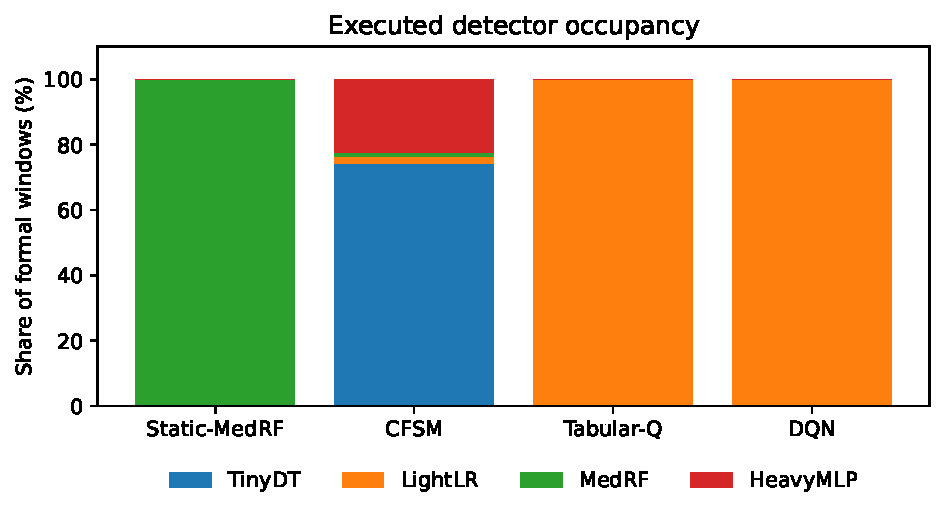
\includegraphics[width=.80\linewidth]{figures/model_occupancy.pdf}
\caption*{\textbf{Figure S1.} Both frozen learned policies execute a constant LightLR schedule. CFSM switches but spends most windows on the poorly performing TinyDT.}
\end{figure}
\begin{figure}[h!]
\centering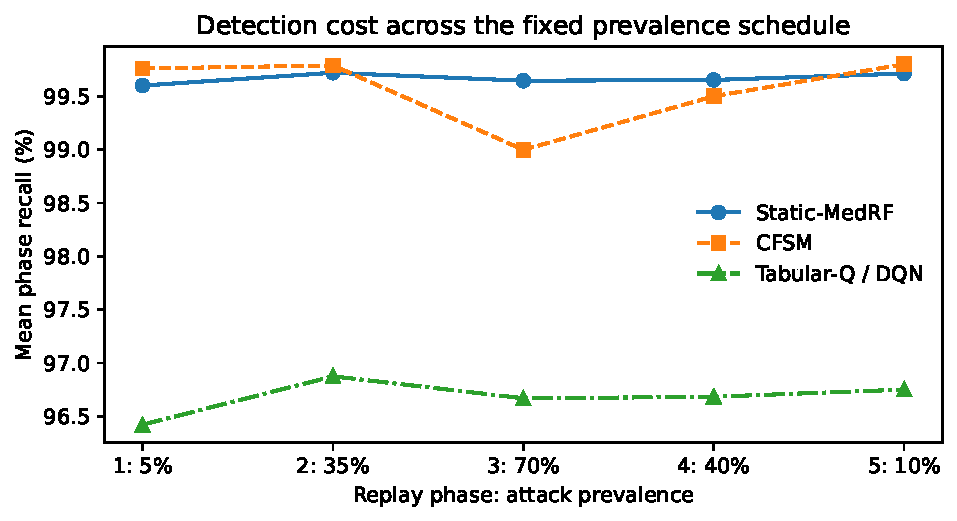
\includegraphics[width=.80\linewidth]{figures/phase_recall.pdf}
\caption*{\textbf{Figure S2.} Mean recall by controlled prevalence phase. Tabular-Q and DQN produce identical selected predictions and are drawn as one series. These phases do not represent newly collected attacks or general concept drift.}
\end{figure}

\clearpage
\section{Policy training and checkpoint selection}
Tabular-Q and DQN each use one policy-training seed, 20260907, with 1,000 software episodes of 500 windows. The ten training traces and five validation traces are source-ID disjoint from the ten test traces. Validation is recorded every 25 episodes. The frozen Tabular-Q checkpoint comes from episode 50 and the DQN checkpoint from episode 25 (one-based numbering), not automatically from the final episode. Full curves, checkpoint metadata, and all 324 reconstructed greedy state actions are retained.

\begin{figure}[h!]
\centering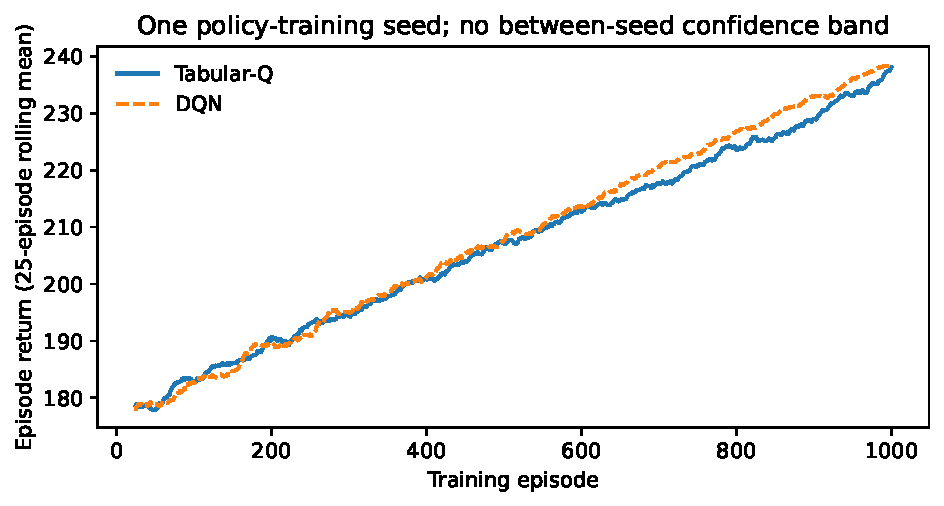
\includegraphics[width=.94\linewidth]{figures/training_returns.pdf}
\caption*{\textbf{Figure S3.} Training returns, displayed with a 25-episode trailing mean. Unsmoothed values are available in CSV. This is one realization per algorithm, not a multi-seed convergence guarantee.}
\end{figure}
\begin{figure}[h!]
\centering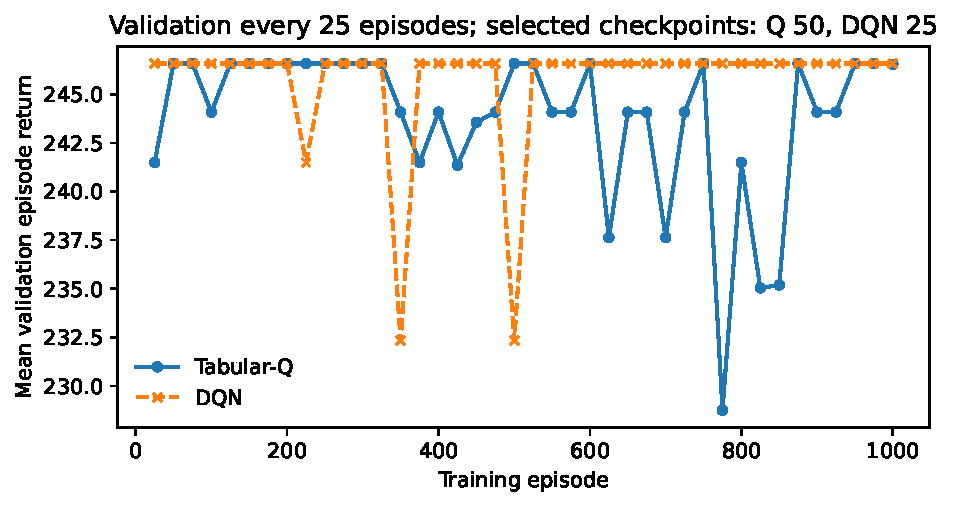
\includegraphics[width=.94\linewidth]{figures/validation_returns.pdf}
\caption*{\textbf{Figure S4.} Recorded validation returns and checkpoint selection. The validation curve is not monotonic; the selected checkpoint is not evidence of convergence of every later iterate.}
\end{figure}

\clearpage
\section{Post-hoc reward and state-coverage diagnostic}
\subsection{Pairwise non-degeneracy criterion}
For two actions $a,b$, write the frozen scalar utility difference as
\[
U_a(s)-U_b(s)=w_D\Delta D_{ab}(s)-\Delta C_{ab},\qquad w_D>0,
\]
where $\Delta C_{ab}$ is the normalized non-detection resource-penalty difference on the declared support, and define $\tau_{ab}=\Delta C_{ab}/w_D$. Then
\[
\operatorname{sign}(U_a(s)-U_b(s))=\operatorname{sign}(\Delta D_{ab}(s)-\tau_{ab}).
\]
Hence strict preference reversal over finite support $\mathcal S$ exists iff
\[
\min_{s\in\mathcal S}\Delta D_{ab}(s)<\tau_{ab}<\max_{s\in\mathcal S}\Delta D_{ab}(s).
\]
If the threshold lies outside this attainable interval, no optimizer can make that pair exchange rank under the frozen scalar utility on that support. With multiple normalized resource terms, $\Delta C_{ab}=\sum_j w_j(\bar C_{j,a}-\bar C_{j,b})$. Candidate-pool min--max scaling therefore makes the implied security--resource exchange rate depend on pool membership; an external power, latency, energy, or thermal budget provides a more stable deployment reference.

\subsection{Executed reward decomposition}
The fixed reward is $0.5\,\mathrm{BA}-0.2\,\widetilde P-0.2\,\widetilde L-0.1\,\widetilde H$. The power min--max span is 0.049806200 W; the batch-latency span is 29.654800 ms. Under the training environment, temperature is held at 35 degrees Celsius and the thermal penalty is zero. The nonthermal resource penalty is 0.001662195 for LightLR and 0.4 for MedRF. Consequently, at equal thermal cost, MedRF requires an immediate balanced-accuracy improvement greater than 0.79667561 to exceed LightLR's single-window reward. This calculation explains the strength of the declared normalization; it is not a proof of a global optimal policy and did not lead to post-test reward changes.

Independent recomputation of the label-informed one-step reference selects LightLR in 4,991 of 5,000 held-out windows and HeavyMLP in nine, with neither MedRF nor TinyDT selected. This is a diagnostic reference using unavailable deployment labels, not a deployable comparison policy. Its CSV retains the objective and selected predictions.

All formal temperature and queue fields map to bin 0, and load maps to bin 1. Threat context varies, but there is no tested high-temperature or high-load region. The frozen DQN selects LightLR in every one of the 324 encoded states; the tabular policy selects LightLR in ten states and TinyDT in 314. Unvisited or zero-initialized tabular entries are not evidence of valid behavior outside the measured support. No thermal model was fitted or validated in this adaptive package, and no such performance is claimed.

\clearpage
\section{Secondary pairwise and state-support diagnostics}
The primary analysis compares each adaptive method with Static-MedRF because that contrast was fixed in the original forty-run matrix. The following pairwise calculations are secondary diagnostics derived from the same ten blocks. They are useful for interpreting the realized policy but are not substituted for the primary endpoint.

\begin{table}[h!]
\centering\small
\caption*{\textbf{Table S12.} Selected secondary paired contrasts from the original campaign. Differences are first method minus second method; intervals use ten block-level Student-$t$ differences.}
\begin{tabular}{llrr}\toprule
Contrast & Metric & Mean difference & 95\% CI\\\midrule
\tableinput{tables/pairwise_secondary_rows}
\bottomrule\end{tabular}
\end{table}

Tabular-Q and DQN have identical selected predictions, so their detection differences are exactly zero rather than statistically estimated near-zero quantities. Tabular-Q nevertheless uses 6.841 J less energy on average than DQN (95\% CI 3.965--9.717 J in Tabular-Q's favor). Tabular-Q also uses 3.123 J less than CFSM (0.785--5.461 J) while producing much higher F1. These empirical mean relations do not identify isolated controller cost and do not generalize beyond the campaign.

\begin{table}[h!]
\centering\small
\caption*{\textbf{Table S13.} Greedy action map and observed state support for the two learned policies. ``All'' counts cover the 324 encoded states; ``Observed'' counts cover unique states reached during the formal learned-policy runs.}
\begin{tabular}{lrrrrrr}\toprule
Method & All states & Observed & All TinyDT & All LightLR & Obs. TinyDT & Obs. LightLR\\\midrule
\tableinput{tables/policy_state_support_rows}
\bottomrule\end{tabular}
\end{table}

Tabular-Q and DQN each reach only four unique states in formal execution. DQN maps every encoded state to LightLR. Tabular-Q maps ten encoded states to LightLR and 314 to TinyDT, but all four states actually reached by the learned-policy runs are LightLR states. Because most tabular states are never visited and many Q entries retain initialization structure, the all-state tabular map is not treated as validated deployment behavior outside observed support.

The phase-level diagnostic reaches the same conclusion. Neither learned policy changes action at a replay-phase boundary. Relative to Static-MedRF, mean learned-policy recall is lower by approximately 2.85--3.18 percentage points across each of the five phases while FPR is lower by approximately 0.16--0.20 percentage points. Phase-varying aggregate metrics therefore describe a constant LightLR operating point under changing class prevalence, not learned phase adaptation.

\section{Archive reconciliation and reproducibility limits}
All 558 top-level adaptive manifest entries verify. The runtime manifest separately references 57 artifacts: 22 match supplied bytes directly, 22 trace index/label arrays are independently reconstructed byte-exactly, seven depend on the frozen external baseline, and six source paths originally differed from the later source copies packaged with the adaptive ZIP. A self-consistent final ZIP and a byte-identical execution snapshot are therefore distinct verification questions.

The six runtime paths are \path{controller.py}, \path{worker.py}, \path{scheduler/artifacts.py}, \path{scheduler/cli.py}, \path{scheduler/evaluation.py}, and \path{scheduler/trace_io.py}. An archival source-recovery package contains all six historically executed byte sequences. Independent verification confirms 6/6 exact SHA-256 matches to the runtime-bound expected values, verifies all 17 content entries in its manifest, and retains later source copies separately. No experiment was rerun and no primary evidence was modified for this closure. The historical primary archive itself does not isolate scheduler decision overhead. That gap is addressed only by the corrected scheduler-overhead microbenchmark described below; source recovery alone does not add measurement evidence.

\clearpage
\section{Matched Static-LightLR physical control}
This is a post-hoc attribution experiment designed after the primary learned policies were observed to select LightLR throughout. It contains ten matched blocks with Static-LightLR, Tabular-Q, DQN, and Static-MedRF. The archive retains 42 attempted runs: 40 valid formal runs, one DQN preparation failure before workload execution, and one Static-MedRF interruption after 403/500 power samples. The interrupted run is linked to exactly one authorized \texttt{retry1} replacement. No invalid attempt is silently deleted or combined with its replacement.

For every valid Tabular-Q, DQN, and Static-LightLR run, the selected-probability hash, confusion counts, and detection metrics are identical within the matched block. Each valid run contains 501 power observations and 500 decisions. Independent trapezoidal reintegration from the raw monotonic timestamps reproduces the registered run energy.

\begin{table}[h!]
\centering\footnotesize
\caption*{\textbf{Table S14.} Matched-control paired effects. Differences are first method minus second method. Exact sign-flip $p$ is a secondary robustness diagnostic; Student-$t$ intervals are the primary uncertainty summary.}
\setlength{\tabcolsep}{3.2pt}
\begin{tabular}{llrrr}\toprule
Contrast & Outcome & Mean & 95\% CI & Sign-flip $p$\\\midrule
\tableinput{tables/p1a_full_paired_rows}
\bottomrule\end{tabular}
\end{table}

The Tabular-Q minus Static-LightLR energy contrast is +0.4555 J with interval $[-1.8609,2.7719]$ J. Because no equivalence margin was predeclared, this is reported only as no resolved directional difference. DQN minus Static-LightLR is +4.5251 J with interval [2.6933, 6.3569] J. Static-MedRF minus Static-LightLR is +12.4706 J [10.6105, 14.3306] J and has higher detection quality. The supplementary campaign therefore shows that direct LightLR accounts for essentially the same detection operating point as both learned policies, while DQN carries an additional whole-device energy premium under the retained runtime.

\begin{figure}[h!]
\centering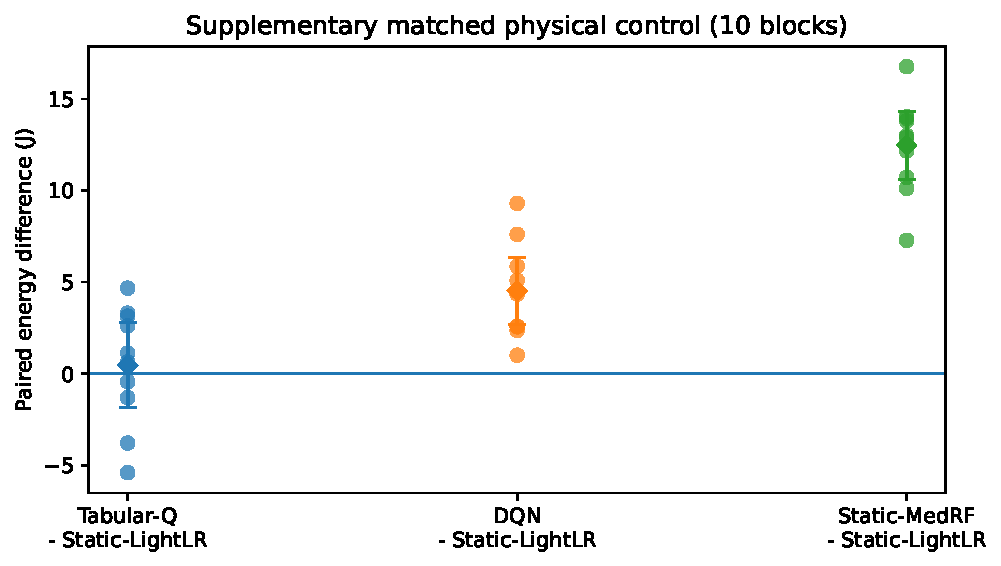
\includegraphics[width=.80\linewidth]{figures/p1a_static_lightlr_energy_control.pdf}
\caption*{\textbf{Figure S5.} Ten matched-control blockwise energy differences with Student-$t$ 95\% intervals.}
\end{figure}

\clearpage
\section{Corrected isolated scheduler-overhead benchmark}
The first scheduler-overhead attempt contained 240 timing units but failed the final validator because its CFSM path substituted fixed MedRF behavior and the required telemetry was absent. The complete attempt remains in the archive and is excluded from inference. A single authorized corrected replacement repeats the frozen benchmark design, adds telemetry, and passes 240/240 units. A deterministic 5,000-state comparison between the corrected CFSM and the frozen rule reports zero action mismatches.

Each method is measured in 30 paired benchmark blocks on each of two state streams: all 324 encoded states and the state support observed in the held-out traces. Each block executes 1,000 warm-up decisions and 10,000 timed state-to-action decisions. The raw nanosecond arrays reproduce the registered mean, median, p95, p99, and sample standard deviation exactly. The repeat unit is the benchmark block, not the 10,000 individual timings.

\begin{table}[h!]
\centering\footnotesize
\caption*{\textbf{Table S15.} Corrected decision overhead. The CI is across 30 block means; p95/p99 are means of block-level quantiles.}
\setlength{\tabcolsep}{3.3pt}
\begin{tabular}{llrrrr}\toprule
Stream & Method & Mean ($\mu$s) & 95\% CI & p95 ($\mu$s) & p99 ($\mu$s)\\\midrule
\tableinput{tables/p1b_all_rows}
\bottomrule\end{tabular}
\end{table}

On observed support the means are 0.739~$\mu$s for Static-LightLR, 6.582~$\mu$s for CFSM, 10.796~$\mu$s for Tabular-Q, and 1.5669 ms for DQN. DQN is about 145 times the Tabular-Q state-to-action time but remains approximately 0.157\% of a one-second decision interval. These timings are not converted into energy.

\begin{figure}[h!]
\centering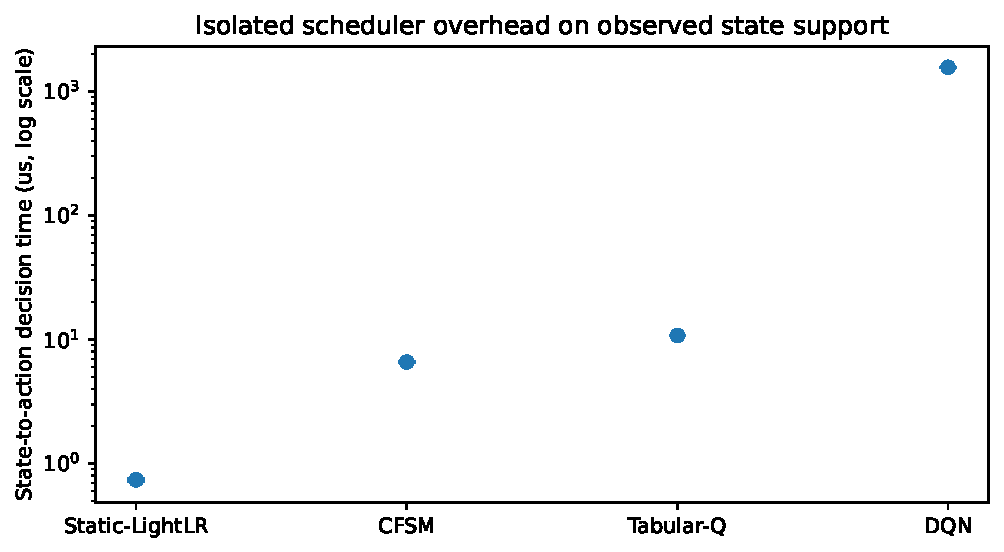
\includegraphics[width=.80\linewidth]{figures/p1b_scheduler_overhead_observed_support.pdf}
\caption*{\textbf{Figure S6.} Corrected state-to-action timing on observed state support. The vertical axis is logarithmic.}
\end{figure}

\clearpage
\section{Multi-seed frozen-policy robustness}
This analysis trains ten additional Tabular-Q and ten additional DQN policies under the frozen state, reward, data split, training horizon, and validation-only checkpoint rule. During final closure, the missing derived validation/test registry is produced from those already frozen checkpoints without retraining or checkpoint reselection. All twenty policies select LightLR in 100\% of held-out windows. Thus each algorithm has 10/10 held-out LightLR collapses, with Wilson 95\% interval [0.7225, 1.0000]. Raw switch counts include one initialization event per held-out trace; between-window switches are zero.

This robustness is support-limited rather than global. The action maps over all 324 encoded states vary across seeds, particularly for DQN. Table S16 reports the complete map counts while the final column reports held-out LightLR occupancy.

\begin{table}[h!]
\centering\footnotesize
\caption*{\textbf{Table S16.} Greedy global action maps and held-out occupancy. Counts cover all 324 encoded states.}
\setlength{\tabcolsep}{3.3pt}
\begin{tabular}{lrrrrrr}\toprule
Algorithm & Seed & TinyDT & LightLR & MedRF & HeavyMLP & Held-out LR (\%)\\\midrule
\tableinput{tables/p1c_global_map_rows}
\bottomrule\end{tabular}
\end{table}

\clearpage
\section{Reward/state and hyperparameter sensitivity}
The reward/state sensitivity analysis contains 85 valid policies plus one retained interrupted DQN attempt. Every valid policy is single-action on held-out support. Of the 85, 80 select LightLR. The only exceptions are the five Tabular-Q \texttt{detection\_only} reward policies, which select MedRF throughout and recover the MedRF-like F1. All thirty Tabular-Q state-ablation policies select LightLR. This supports specification sensitivity in a precise sense: the tested resource-aware objectives and state removals preserve the LightLR operating point, while deleting all resource penalties changes which static detector is preferred.

\begin{table}[h!]
\centering\footnotesize
\caption*{\textbf{Table S17.} Held-out reward/state policy results by family/variant. ``LR'' is the number of LightLR-collapsed policies; ``Single'' counts any single-action policy.}
\setlength{\tabcolsep}{3.2pt}
\begin{tabular}{lllrrrr}\toprule
Family & Algorithm & Variant & $n$ & LR & Single & Mean F1\\\midrule
\tableinput{tables/p1d_rows}
\bottomrule\end{tabular}
\end{table}

The hyperparameter analysis contains 35 valid Tabular-Q runs over the predeclared discount/learning-rate matrix. All 35 select LightLR throughout held-out support and are single-action. These results are sensitivity evidence only; none is used to choose a replacement primary hyperparameter after test inspection.

\begin{table}[h!]
\centering\footnotesize
\caption*{\textbf{Table S18.} Tabular-Q hyperparameter sensitivity on held-out support.}
\begin{tabular}{lrrrr}\toprule
Variant & $n$ & LR & Single & Mean F1\\\midrule
\tableinput{tables/p1e_rows}
\bottomrule\end{tabular}
\end{table}

\clearpage
\section{Fixed-rate confidence cascade}
The fixed-rate campaign contains 40 valid 500-second runs in ten paired blocks. Static-LightLR, the frozen Tabular-Q policy, Static-MedRF, and the confidence cascade use the same trace within block; every method has an immediately preceding idle segment. The cascade band is fixed at $[0.3,0.7]$ and ground truth is never used for escalation. It sends 1.3388\% of rows to MedRF.

\begin{table}[h!]
\centering\footnotesize
\caption*{\textbf{Table S19.} Fixed-rate method means. Adjusted power subtracts the immediately preceding idle.}
\setlength{\tabcolsep}{3.0pt}
\begin{tabular}{lrrrrrrr}\toprule
Method & Energy & Power & Adjust. & F1 & Recall & FPR & Esc.\\
 & (J) & (W) & (mW) & & (\%) & (\%) & (\%)\\\midrule
\tableinput{tables/r1_revision_rows}
\bottomrule\end{tabular}
\end{table}

Against Static-LightLR, paired cascade effects are +7.952 J [5.897,10.007], +15.917 raw mW [11.798,20.035], and +13.635 idle-adjusted mW $[-1.515,28.784]$. F1/recall/FPR differences are +1.347/+2.676/+0.018 percentage points. The raw and adjusted results are both retained because the adjusted interval indicates sensitivity to ambient/carryover drift.

The frozen worker implements sub-batch escalation, not one MedRF call per deferred row: it evaluates LightLR on the full 100-row batch and invokes MedRF once on the subset satisfying $0.3\le p_{LR}\le0.7$. The apparently disproportionate latency is explained by call granularity. Only 1.3388\% of rows are deferred, but they occur in 66.76\% of windows; among those windows the mean deferred subset has only 2.01 rows. A no-defer window averages 1.636 ms, whereas any-defer windows average 31.884 ms, nearly independent of whether one or several rows are deferred. Thus the 21.830-ms overall mean reflects frequent small MedRF calls at this 100-row cadence rather than row-by-row execution. It is an implementation/operating-point result, not a general bound for optimized cascades.

\begin{table}[h!]
\centering\footnotesize
\caption*{\textbf{Table S19a.} Confidence-cascade call-granularity diagnostic reconstructed from 5,000 frozen window logs.}
\begin{tabular}{lr}\toprule
Quantity & Value\\\midrule
\tableinput{tables/r1_cascade_latency_decomposition_rows}
\bottomrule\end{tabular}
\end{table}

\begin{figure}[h!]
\centering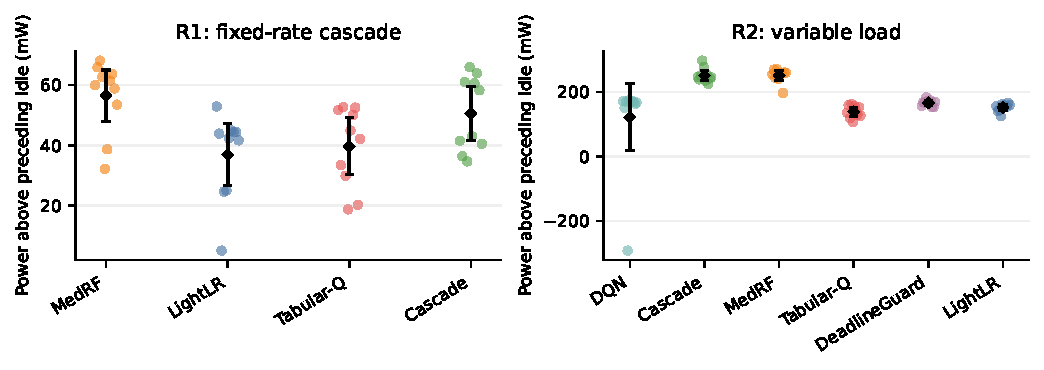
\includegraphics[width=.95\textwidth]{figures/revision_drift_adjusted_power.pdf}
\caption*{\textbf{Figure S7.} Preceding-idle-adjusted power across fixed-rate and variable-load campaigns. Small points are runs; diamonds and bars are method means and Student-$t$ 95\% intervals over runs. Pairwise inference uses within-block differences in the CSV, not these marginal intervals.}
\end{figure}

\clearpage
\section{Variable-load factorial and DeadlineGuard}
Each of the 60 valid runs visits every 50/100/4000 rows/s $\times$ 0.10/0.50/0.90 prevalence cell exactly once, then the fixed recovery cell. The controller sees causal measurements rather than cell identity. Static-MedRF misses 512 of 5,000 deadlines and Cascade misses 21; DeadlineGuard and the remaining methods miss none. All final backlogs are zero, so deadline misses and end-of-run backlog are distinct endpoints.

\begin{table}[h!]
\centering\footnotesize
\caption*{\textbf{Table S20.} Variable-load method results over ten blocks. Energy is mean$\pm$SD across physical runs; completion is seconds.}
\setlength{\tabcolsep}{2.6pt}
\begin{tabular}{lrrrrrrr}\toprule
Method & Energy & Power & F1 & Recall & FPR & Miss & p95\\
 & (J) & (W) & & (\%) & (\%) & (\%) & (s)\\\midrule
\tableinput{tables/r2_revision_rows}
\bottomrule\end{tabular}
\end{table}

\begin{table}[h!]
\centering\scriptsize
\caption*{\textbf{Table S21.} Variable-load paired effects against Static-LightLR. Energy and adjusted-power intervals use ten within-block differences. F1 is percentage points; $p$ is the exact two-sided sign-flip diagnostic for energy.}
\setlength{\tabcolsep}{2.5pt}
\begin{tabular}{lrrrr}\toprule
Method & $\Delta E$ (J), 95\% CI & $\Delta P_{adj}$ (mW), 95\% CI & $\Delta$F1 & $p$\\\midrule
\tableinput{tables/r2_paired_lightlr_rows}
\bottomrule\end{tabular}
\end{table}

\begin{table}[h!]
\centering\scriptsize
\caption*{\textbf{Table S22.} Variable-load state/action and service evidence. Occupancy totals 5,000 windows/method. Switch counts include the implementation's initialization convention.}
\setlength{\tabcolsep}{2.2pt}
\begin{tabular}{lrlrrrr}\toprule
Method & States & Action occupancy & Switches & Fallback & Misses & Backlog\\\midrule
\tableinput{tables/r2_state_coverage_rows}
\bottomrule\end{tabular}
\end{table}

DeadlineGuard selects MedRF in 3,500 and LightLR in 1,500 windows and records 5.3 switches/run. Against Static-MedRF it uses 43.714 J less per run [41.418,46.010], reduces deadline misses by 10.24 percentage points to zero, and loses 1.373 F1 pp. Frozen DQN remains LightLR. Frozen Tabular-Q selects TinyDT in all 5,000 windows. The registry calls these selections ``fallback'', but the frozen source contains no separate exception branch: unseen zero-initialized Q rows are tied, NumPy argmax chooses the first maximum, and the action order places TinyDT first. The variable-load behavior is therefore the direct hardware realization of the off-support tie/default already visible in the 314/324 TinyDT full greedy map.

DQN's raw energy difference from Static-LightLR is positive in all ten blocks, with median +5.72 J, but Block 4 is +392.0 J and raises the SD of paired differences to 122.2 J; the Student-$t$ 95\% interval consequently spans $[-43.2,131.7]$ J. The same run has a 3.919-W preceding idle and 49.2$^\circ$C maximum temperature. Preceding-idle-adjusted power does not resolve a DQN--LightLR difference. We therefore retain both the 10/10 raw direction (exact sign-flip $p=0.00195$) and the unstable magnitude rather than collapsing them into an ``equivalent'' or causal controller-power claim.

\begin{figure}[h!]
\centering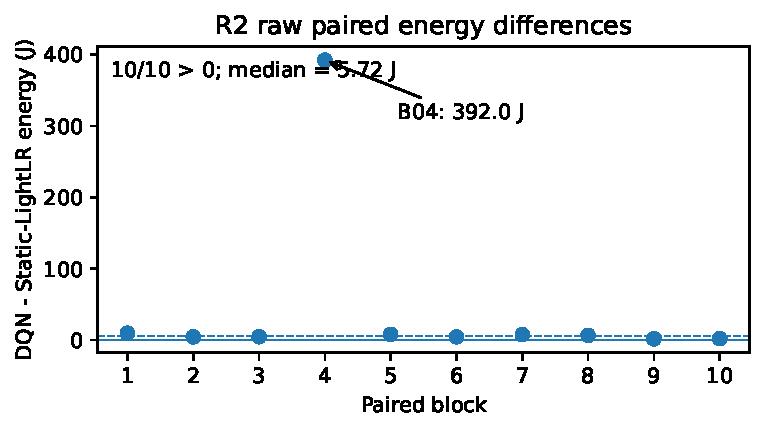
\includegraphics[width=.75\textwidth]{figures/r2_dqn_block_energy_differences.pdf}
\caption*{\textbf{Figure S8a.} DQN-minus-Static-LightLR raw energy by paired block. Nine differences are between 1.8 and 9.6 J; Block 4 is a 392.0-J power/temperature excursion.}
\end{figure}

\begin{figure}[h!]
\centering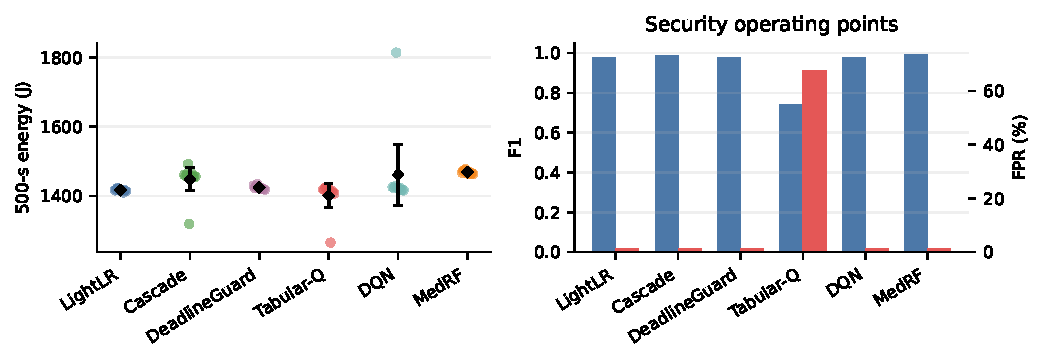
\includegraphics[width=.95\textwidth]{figures/r2_energy_security.pdf}
\caption*{\textbf{Figure S8.} Variable-load raw energy distributions and security operating points. The block is the repeat unit.}
\end{figure}

\clearpage
\section{Protocol stop and TinyDT threshold diagnostic}
The planned controller-only power arm required four original observed-support states for controller-only whole-device measurement. The frozen source exposes eight and contains no outcome-independent rule for selecting four. The campaign therefore stopped before measurement. No controller-only power or joule value is inferred from the scheduler-overhead timing benchmark.

The TinyDT diagnostic selects threshold 0.6467505097 solely on validation balanced accuracy with the highest-threshold tie rule, freezes its hash, and applies it once to test. The optional fixed reference-load check is not executed because an independent stable reference load is unavailable.

\begin{table}[h!]
\centering\footnotesize
\caption*{\textbf{Table S23.} TinyDT test operating point at the primary and diagnostic thresholds. The diagnostic does not replace the primary.}
\setlength{\tabcolsep}{3.0pt}
\begin{tabular}{lrrrrrrrrr}\toprule
Result & $\tau$ & TN & FP & FN & TP & F1 & Rec. & FPR & BA\\\midrule
\tableinput{tables/r4_threshold_rows}
\bottomrule\end{tabular}
\end{table}

The diagnostic changes test F1 from 0.4792 to 0.9698 and FPR from 67.78\% to 1.82\% while recall changes from 99.76\% to 99.61\%. Test AUROC is 0.9906. This supports calibration/threshold sensitivity as an explanation for much of the threshold-0.5 failure, but the analysis was introduced after the discrepancy was known and cannot repair frozen policy outcomes.

\begin{figure}[h!]
\centering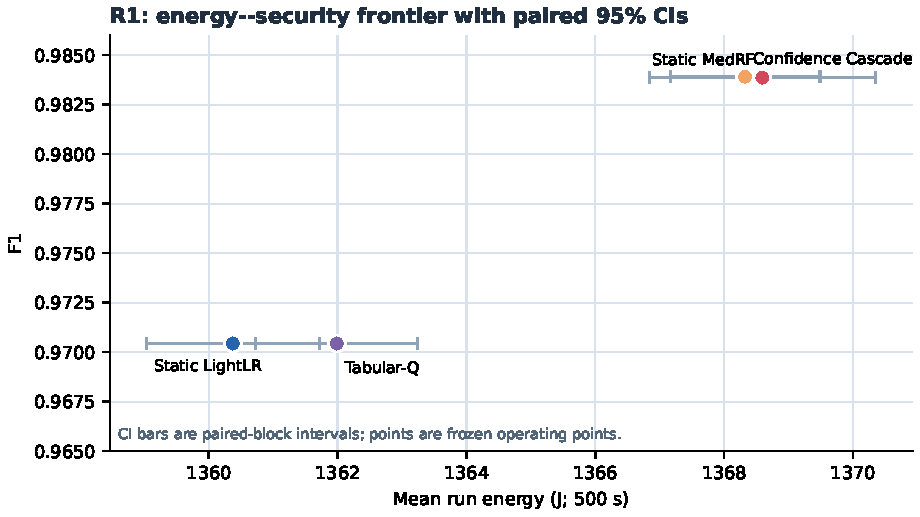
\includegraphics[width=.95\textwidth]{figures/r1_energy_security_frontier.pdf}
\caption*{\textbf{Figure S9.} Fixed-rate energy--security frontier. Horizontal bars are paired-block 95\% CIs for run energy; the plotted F1 values are method means.}
\end{figure}

\begin{figure}[h!]
\centering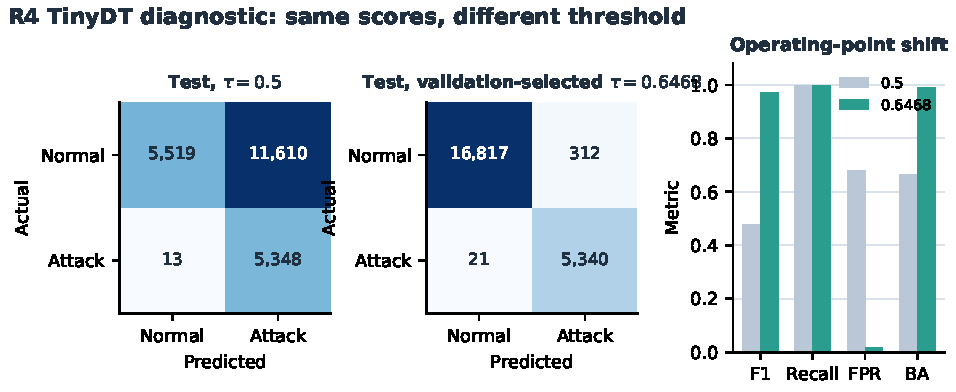
\includegraphics[width=.95\textwidth]{figures/r4_threshold_shift.pdf}
\caption*{\textbf{Figure S10.} TinyDT threshold diagnostic. The primary threshold remains 0.5; the validation-selected threshold is a post-hoc diagnostic only.}
\end{figure}

\clearpage
\section{Recent literature context (2024--2026)}
The main text now cites twenty recent peer-reviewed studies from CCF-A or CCF-B venues. The entries are deliberately used as contextual comparators rather than as evidence for this experiment's physical claims. Their common themes are edge orchestration, energy/deadline trade-offs, learning-based control, and robust offloading/caching. Venue classification follows the CCF 2022 journal catalogue (TMC=A; TSC=A); publication metadata and DOI links are retained in \texttt{references.bib}. None of these studies changes the frozen detector artifacts, split, thresholds, or physical measurements reported here.

\begin{table}[h!]
\centering\scriptsize
\caption*{\textbf{Table S24.} Added 2024--2026 literature set. All entries are IEEE Transactions on Mobile Computing (CCF-A) except Zhang \emph{et al.}, IEEE Transactions on Services Computing (CCF-A).}
\begin{tabular}{p{.52\textwidth}ll}
\toprule
Topic & Years & Keys\\\midrule
DVFS, startup-aware scheduling, distributed offloading & 2024 & \cite{Zhang2024DVFO,Lou2024Startup,Kim2024DistributedOffload}\\
Robust caching, dependency-aware and incentive-aware offloading & 2024 & \cite{Chen2024ABR,Feng2024PRAISE,Tutuncuoglu2024Serverless,Hu2024MICDA}\\
QoS, trust, D2D and random-access edge control & 2024--25 & \cite{Maleki2024QCS,Wang2025TrustOffload,Hu2025SITOff,Han2025OffloadingGame}\\
Energy harvesting, satellite/UAV/vehicular coordination & 2024--25 & \cite{Zhang2024Satellite,Luo2025SolarEdge,Gong2025UAV3D,Zhao2025COHCTO}\\
Digital-twin inference, distributed coding, uncertain inference, and edge caching & 2024--26 & \cite{Zhang2024AoI,Qiu2026Barycentric,Nan2026RobustDNN,Luo2025EdgeCache,Li2024FIMI}\\
\bottomrule
\end{tabular}
\end{table}

\section{Evidence archive integrity}
The strengthening evidence archive has SHA-256:
\begin{center}\small\texttt{d4e1e96960f1279c79445c744a02be1033e288dad27f440b87753934a3f4b108}\end{center}
Its size is 141,322,551 bytes and it contains 1,918 ZIP entries. Its root manifest contains 1,917 entries and independently covers every content file except itself; CRC, manifest, nested-manifest, and final validator checks pass. The reviewer-control evidence archive has SHA-256:
\begin{center}\small\path{845ced5c96f932ee8d3509e2effcb39870a2fb9995bad9a6fe524f6c60b270e4}\end{center}
It has 1,912 entries and a 1,911-file root manifest. Its final validator reports data-lineage, fixed-rate, variable-load, and threshold checks PASS, with the controller-only arm retained as a predeclared-ambiguity stop, no policy retraining, no test-driven selection, and retained invalid/replacement linkage. These properties establish internal provenance, not external validity.
\clearpage
\bibliographystyle{IEEEtran}
\bibliography{references}
\end{document}
